\documentclass{article}
\usepackage{tikz}
\usetikzlibrary{positioning}

\begin{document}
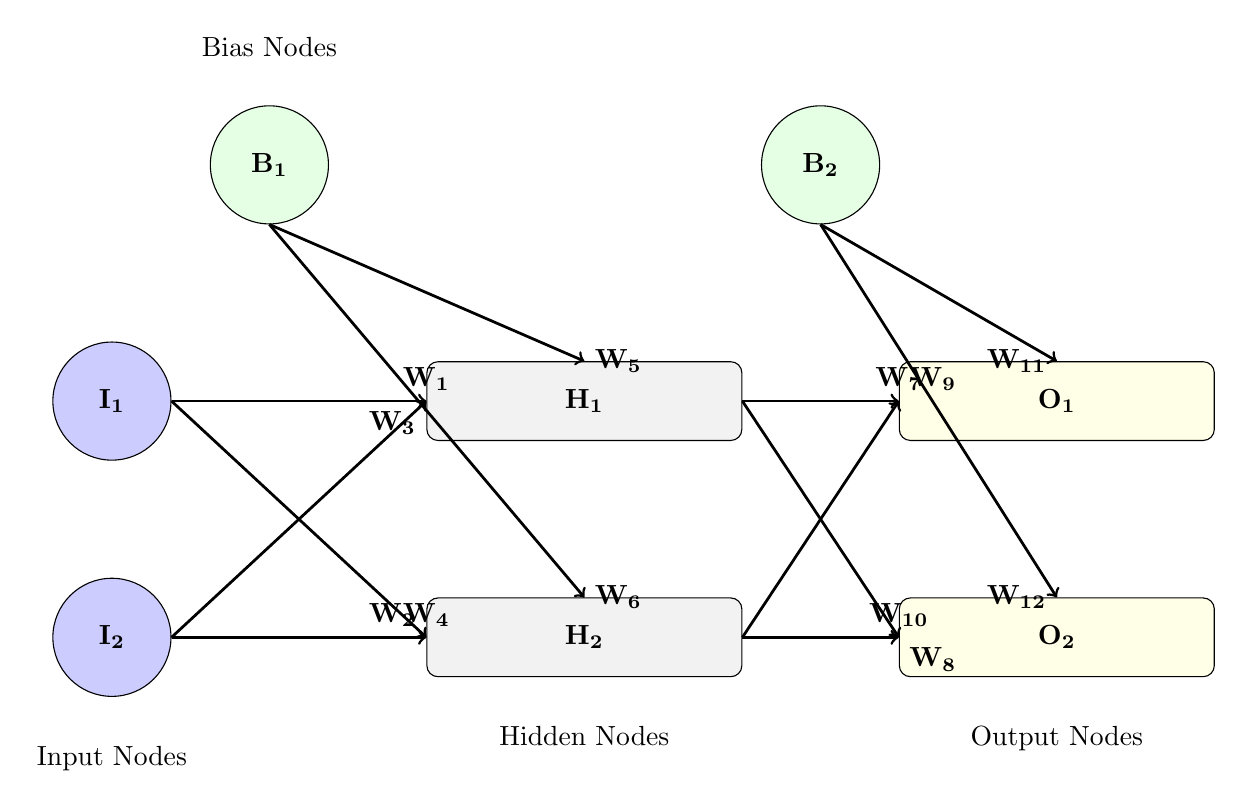
\begin{tikzpicture}
\tikzset{
    bias/.style={circle, draw, minimum size=1.5cm, fill=green!10},
    input/.style={circle, draw, minimum size=1.5cm, fill=blue!20},
    hidden/.style={rectangle, draw, rounded corners, minimum height=1cm, minimum width=4cm, fill=black!5},
    output/.style={rectangle, draw, rounded corners, minimum height=1cm, minimum width=4cm, fill=yellow!10},
    every node/.style={text centered},
    edge/.style={->, line width=1pt}, 
    weight/.style={above, font=\bfseries}
}

% Розміщення вузлів вручну
\node[bias] (B1) at (0,0) {$\mathbf{B_1}$};
\node[bias] (B2) at (7,0) {$\mathbf{B_2}$};
\node[input] (I1) at (-2,-3) {$\mathbf{I_1}$};
\node[input] (I2) at (-2,-6) {$\mathbf{I_2}$};
\node[hidden] (H1) at (4,-3) {$\mathbf{H_1}$};
\node[hidden] (H2) at (4,-6) {$\mathbf{H_2}$};
\node[output] (O1) at (10,-3) {$\mathbf{O_1}$};
\node[output] (O2) at (10,-6) {$\mathbf{O_2}$};

% Підписи для груп вузлів
\node[above=0.5cm of B1] {Bias Nodes};
\node[below=0.5cm of I2] {Input Nodes};
\node[below=0.5cm of H2] {Hidden Nodes};
\node[below=0.5cm of O2] {Output Nodes};

% Стрілки та ваги між вузлами (з використанням node.center для точнішого позиціонування)
\draw[edge] (I1.east) -- (H1.west) node[weight] {$\mathbf{W_1}$};
\draw[edge] (I1.east) -- (H2.west) node[weight, above left] {$\mathbf{W_2}$};
\draw[edge] (I2.east) -- (H1.west) node[weight, below left] {$\mathbf{W_3}$};
\draw[edge] (I2.east) -- (H2.west) node[weight] {$\mathbf{W_4}$};

\draw[edge] (B1.south) -- (H1.north) node[weight, right] {$\mathbf{W_5}$};
\draw[edge] (B1.south) -- (H2.north) node[weight, right] {$\mathbf{W_6}$};

\draw[edge] (H1.east) -- (O1.west) node[weight] {$\mathbf{W_7}$};
\draw[edge] (H1.east) -- (O2.west) node[weight, below right] {$\mathbf{W_8}$};
\draw[edge] (H2.east) -- (O1.west) node[weight, above right] {$\mathbf{W_9}$};
\draw[edge] (H2.east) -- (O2.west) node[weight] {$\mathbf{W_{10}}$};

\draw[edge] (B2.south) -- (O1.north) node[weight, left] {$\mathbf{W_{11}}$};
\draw[edge] (B2.south) -- (O2.north) node[weight, left] {$\mathbf{W_{12}}$};
\end{tikzpicture}
\end{document}
